\chapter{典型应用观测与画像分析}\label{chap:profiling}

\section{云场景典型应用选择}

% 软件环境复杂 -> 应用需求不同 -> 软件架构复杂 -> 存在共性的基础应用 -> 基础应用的性能是整体性能的关键 -> 选取典型应用进行分析

数据中心软件环境复杂,同时托管的应用种类较为丰富,为画像分析带来了许多挑战。首先,数据中需要根据用户的使用需求,提供不同的软件环境,如针对虚拟机,需要提供虚拟化环境,而对于容器,则需要提供如K8s等,本研究结合与云厂商的合作经验,选择云场景中使用较普遍的虚拟机作为目标场景,在该场景中,应用的运行环境由宿主机系统、虚拟化运行时及来宾操作系统共同完成。其次,数据中心托管应用丰富的主要原因是需求的差异,然而当前随软件架构的不断进步及开源、云原生等理念的推广,应用在设计时会使用到许多相同的公共组件,如数据库、消息中间件等,这些公共组件构成了现代软件的基石,同时也是应用性能的关键,因此在本研究中,结合与云厂商的合作经验,从传统数据库、键值存储、消息中间件、大数据、媒体处理等领域中选择了如表~\ref{tab:typical_application}所示的7种典型应用进行画像分析。

\begin{table}
    \bicaption{\quad 云场景典型应用}{\quad Typical Applications in Cloud Scenarios}% caption
    \label{tab:typical_application}
    \footnotesize% fontsize
    \setlength{\tabcolsep}{4pt}% column separation
    \renewcommand{\arraystretch}{1.5}% row space 
    \centering
    \begin{tabular}{lc}
        \hline
        %\multicolumn{num_of_cols_to_merge}{alignment}{contents} \\
        %\cline{i-j}% partial hline from column i to column j
        类型 & 应用\\
        \hline
        SQL & mysql\\
        NoSQL & elasticsearch\\
        Web Server & nginx\\
        K-V Store & redis、memcached\\
        Message Queue & kafka\\
        Media & render\\
        \hline
    \end{tabular}
\end{table}

这些应用在领域上的差异,决定了其在功能实现上的不同,并会使用到不同的资源,因此各自对调度有不同的需求:

1)数据库类型的应用,如Mysql,传统的关系型数据库提供了完善了数据存储、检索查询及事务管理等功能,实现中原始数据通常保存在磁盘上,在进行大量数据查询时,不仅会使用到较多的CPU资源,同时也会占用相当的IO资源,因此需要调度器保障其CPU资源,并避免IO上的干扰。

2)键值存储类应用,如Redis、Memcached,通常作为信息缓存服务,提供快速的数据存储与查询,由于数据存储在内存中,因此对内存资源存在较高要求,对调度的需求主要体现在两方面,一方面需要足够的内存资源,另一方面则需要避免在内存带宽上的干扰。

3)网络服务类型应用,如Nginx,网络页面通常都具有交互属性,而延迟会极大影响用户的使用体验,因此这类应用要求调度能够在网络请求到达时,及时的为网络服务分配CPU,以尽早地对连接进行处理。

4)媒体处理应用,如ffmjpeg,通常是离线应用,运行时会占用大量的CPU资源,来进行编解码操作,这类应用需要调度分配足够长的时间片,同时希望能减少上下文地切换,以便更好地利用局部性来加快执行速度。

\section{观测系统设计与指标收集}

\subsection{面向虚拟机的多维指标采集设计}

% 分解虚拟机: Host侧 -> Hypervisor侧 -> 应用侧
% 分解采集系统:
% - 采集侧
% - 查询、存储、分析侧

本研究中使用KVM虚拟机作为混部应用基本软件环境。而结合第二章中对于虚拟化沙箱技术的分析,本研究设计了一种如图~\ref{fig:virtualmachine}所示的面向虚拟机的多维度指标采集机制。

\begin{figure}[!htbp]
    \centering
    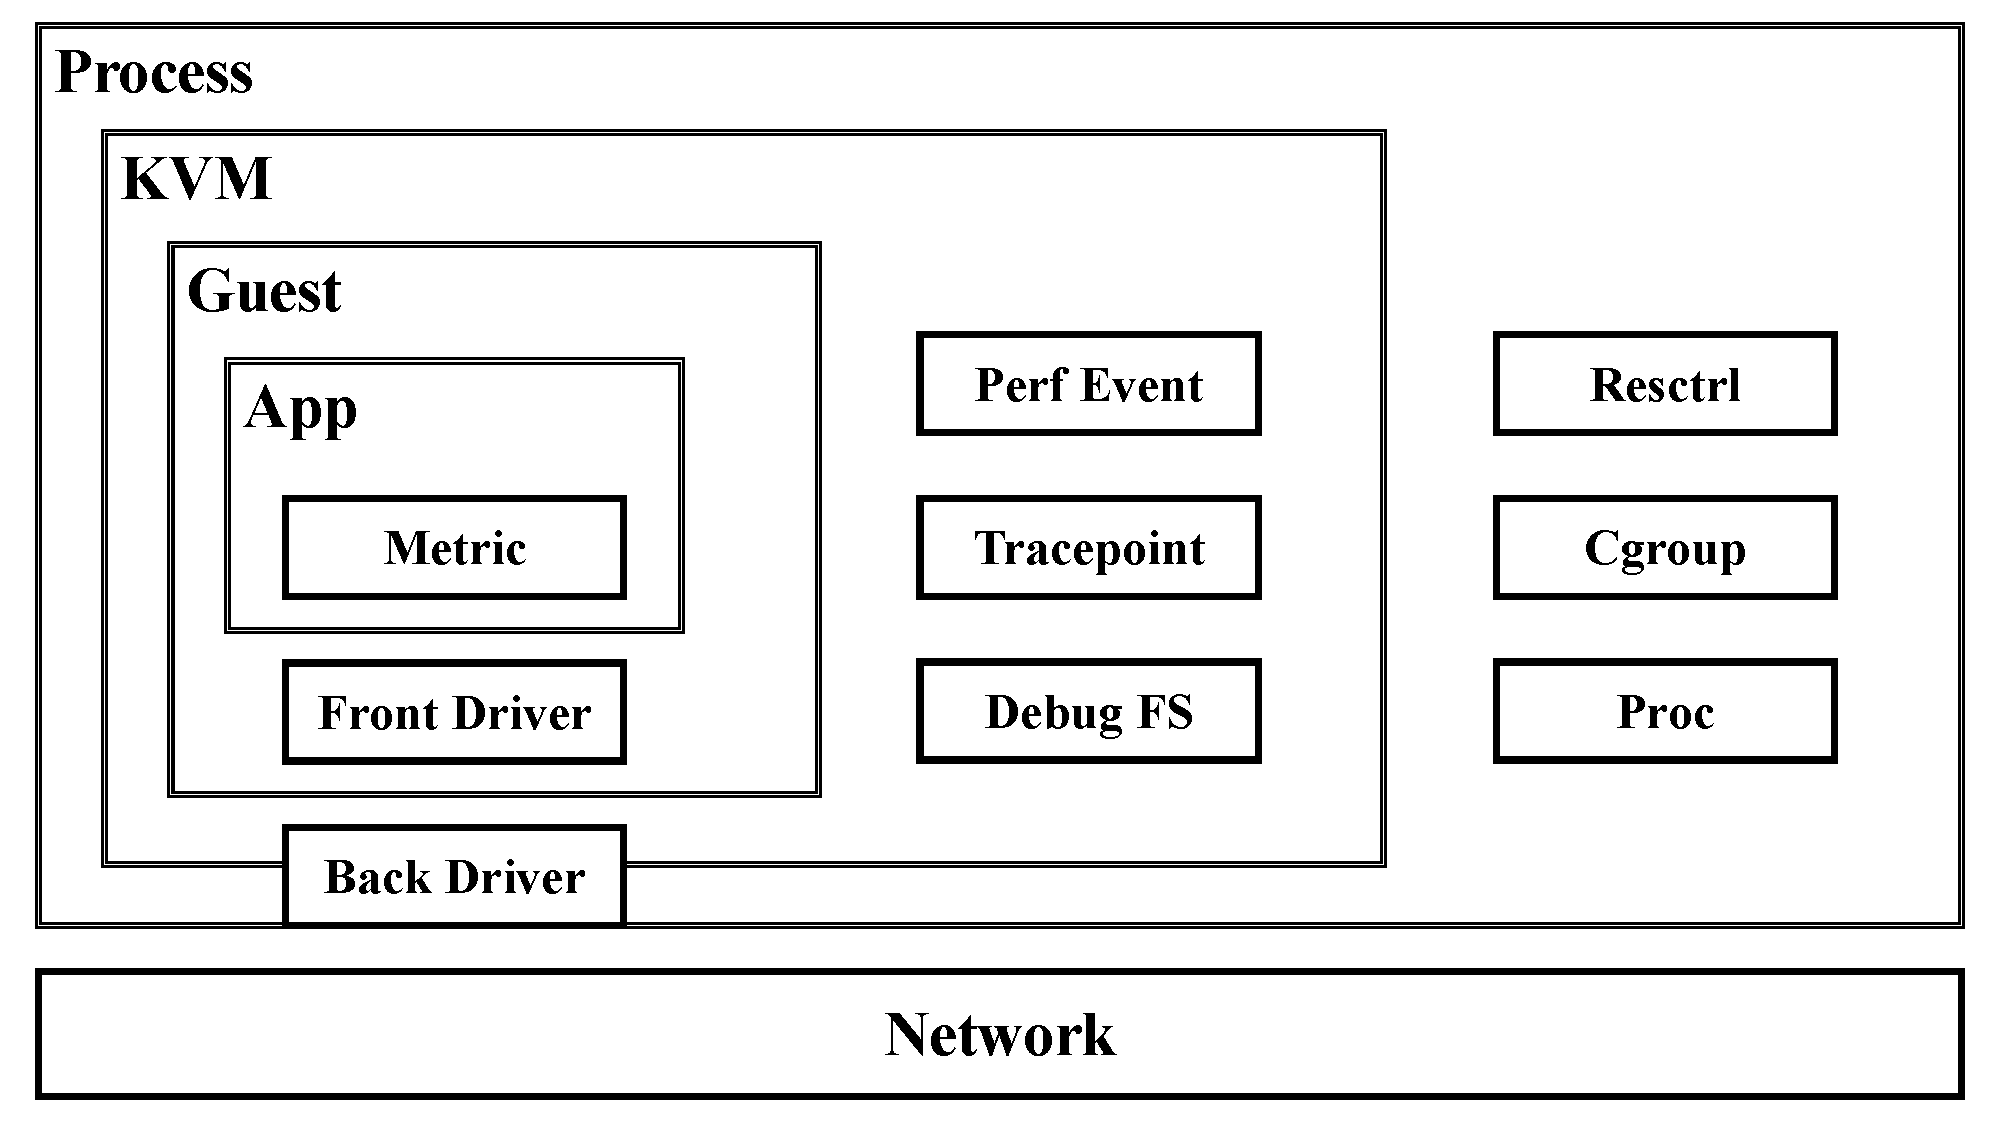
\includegraphics[width=0.7\textwidth]{virtualmachine}
    \bicaption{\quad 虚拟机多维度指标采集}{\quad Multi-dimensional metrics from virtual machines}
    \label{fig:virtualmachine}
\end{figure}

首先,在宿主机上,KVM虚拟机由多个进程组成,因此在这一维度,可以利用宿主机Kernel提供的多种进程监测机制,如/proc内核文件系统中记录的进程信息,以及cgroup子系统中对进程的记账信息,来评测虚拟机进程的性能。其次,虚拟机由各个模拟硬件组成,这些设备由Hypervisor进行模拟,在此维度,能够利用Hypervisor提供的丰富接口,来获取虚拟机的各个虚拟机设备的性能信息,以vCPU为例,本研究中KVM内核模块负责虚拟机的vCPU模拟,而KVM内核模块通过debug文件系统提供了丰富的vCPU监测信息,如包括IO、挂起、中断等在内的陷出计数,以及MMU缓存缺失计数等。最后,虚拟化环境最终需要为应用的运行提供服务,应用级指标能够体现出应用的真实性能,而针对这一维度的指标采集,主要从两个方面入手,对于Client-Server类的服务型应用,可以在外部通过Overlay网络建立对延迟、吞吐量的追踪,部分应用也内置了观测接口,提供性能信息的采集。

而为更深入地探测虚拟机性能,本研究还基于eBPF设计了一种在内核侧监测的机制。首先,在宿主机维度,进程对于硬件资源的使用通常都需要通过系统调用完成, 如使用网络资源时,需要使用send或recv系统调用,使用IO资源时,需要进行read、write系统调用,对虚拟机而言,这种方式能够监测陷出到用户态之后的设备模拟过程。其次,在Hypervisor维度,为追求设备模拟的效率,一些模拟硬件的后端实现并不要求虚拟机陷出到用户态,而直接在内核态完成整个模拟过程,如图~\ref{fig:vhost_net}所示,vHost net作为一种内核态实现的模拟网络设备后端,其网络发送的过程就直接在内核中通过函数调用进行,而这些函数的执行状态能够反映出模拟网络设备后端的性能。

\begin{figure}[!htbp]
    \centering
    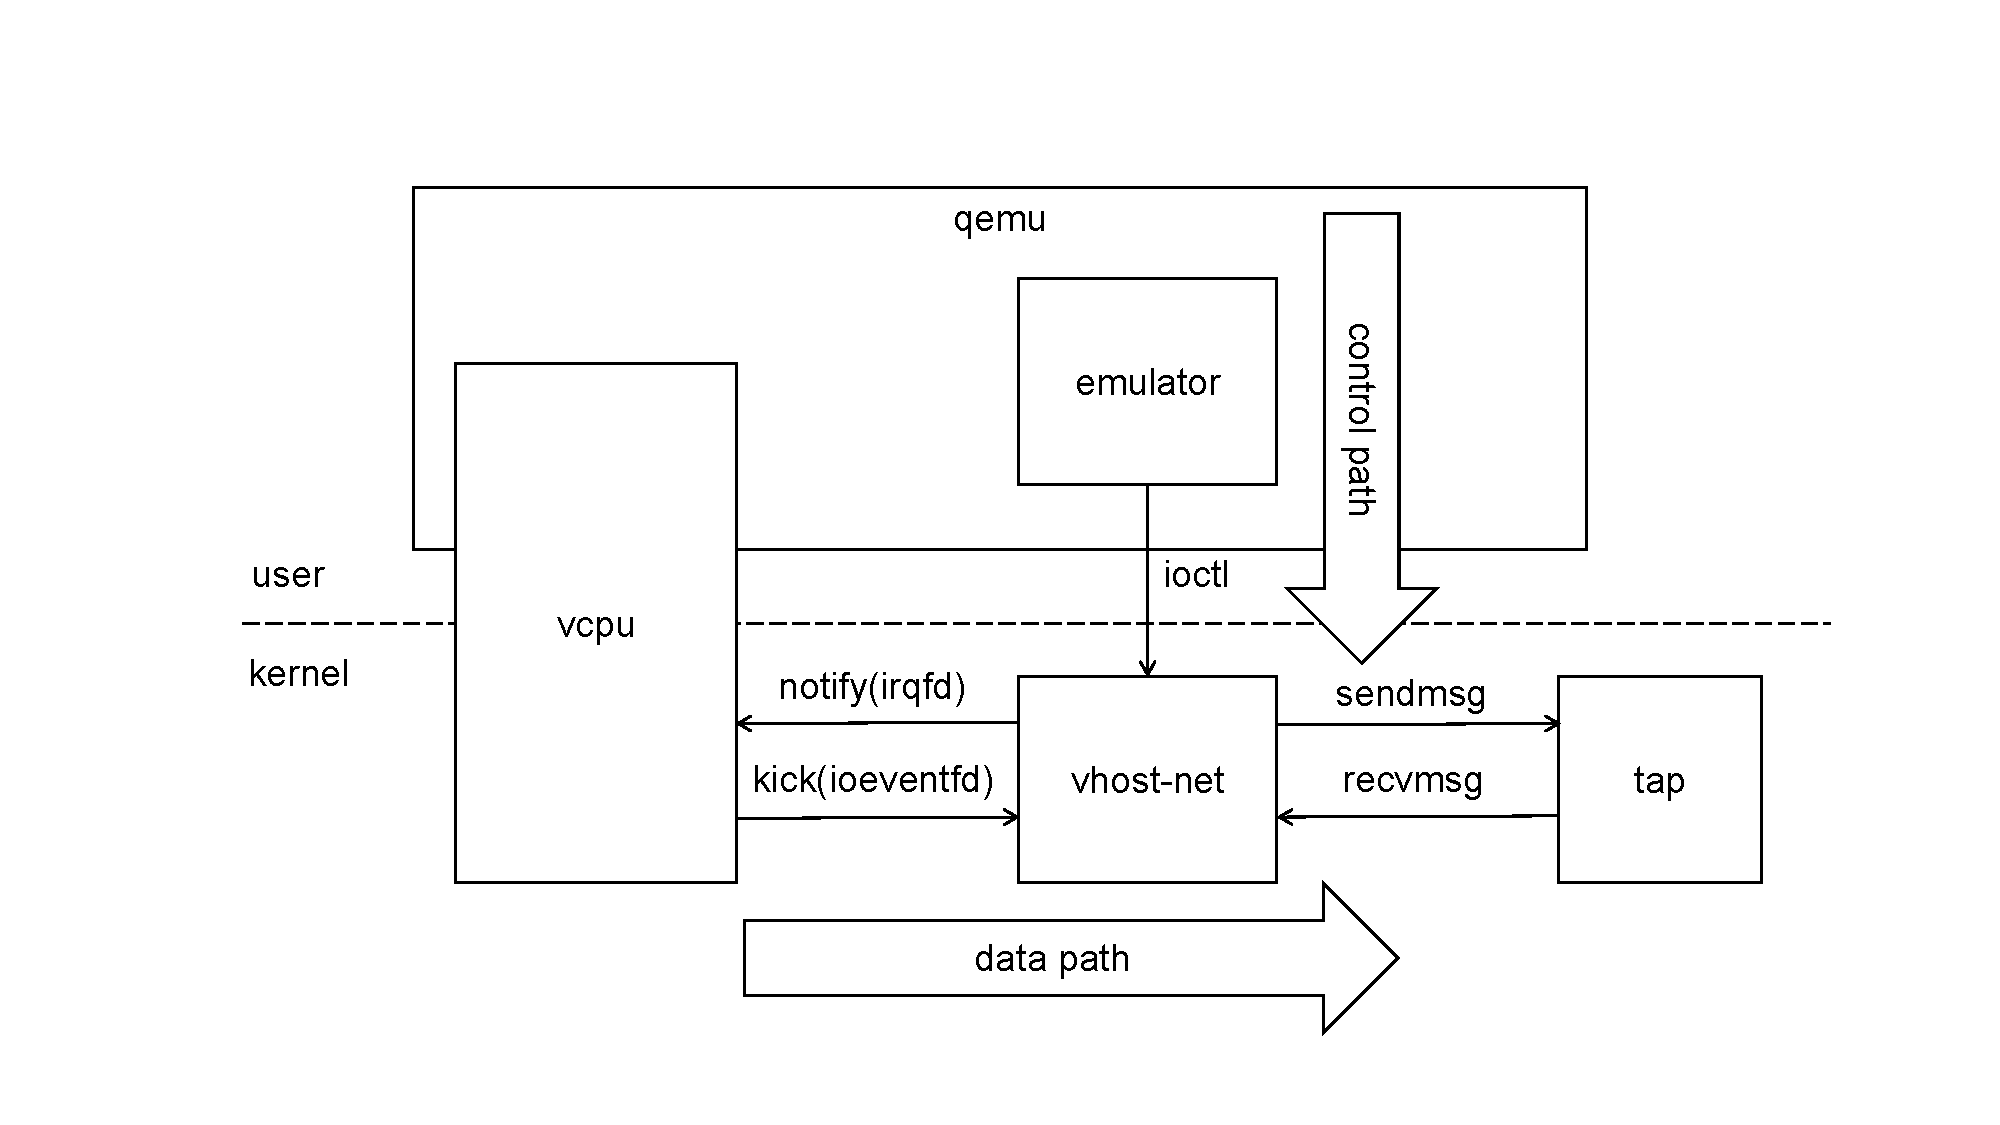
\includegraphics[width=0.7\textwidth]{vhost_net}
    \bicaption{\quad vHost Net模拟网络设备后端}{\quad vHost Net Simulate network device backend}
    \label{fig:vhost_net}
\end{figure}

综合以上分析,本研究设计了一种实时指标采集分析系统,能从上述维度以虚拟机为粒度机进行指标采集,同时能够提供指标的存储、查询与分析服务。系统中定义了Observer与Observed两种角色,首先,Observer与Observed以统一的格式对指标进行编解码,随后,Observed中部署监控组件以对外部提供监控服务,最后,Observer周期性地轮询各个Observed,并将收集到的原始指标按标签进行区分存储,并根据预定义的规则对指标进行聚合处理,同时对外提供查询与分析服务。系统中可以有多个Observer来分摊采集压力,并且每个节点可以按需要同时承担Observer与Observed两种角色。

\subsection{实时可观测性系统实现}

% Observer实现
% - Prometheus、Grafana、Collector Utils
% Observed实现
% - Exporter的实现细节
%   - Ebpf Exporter
%       - Syscall 追踪
%       - vHost Net 追踪

\begin{figure}[!htbp]
    \centering
    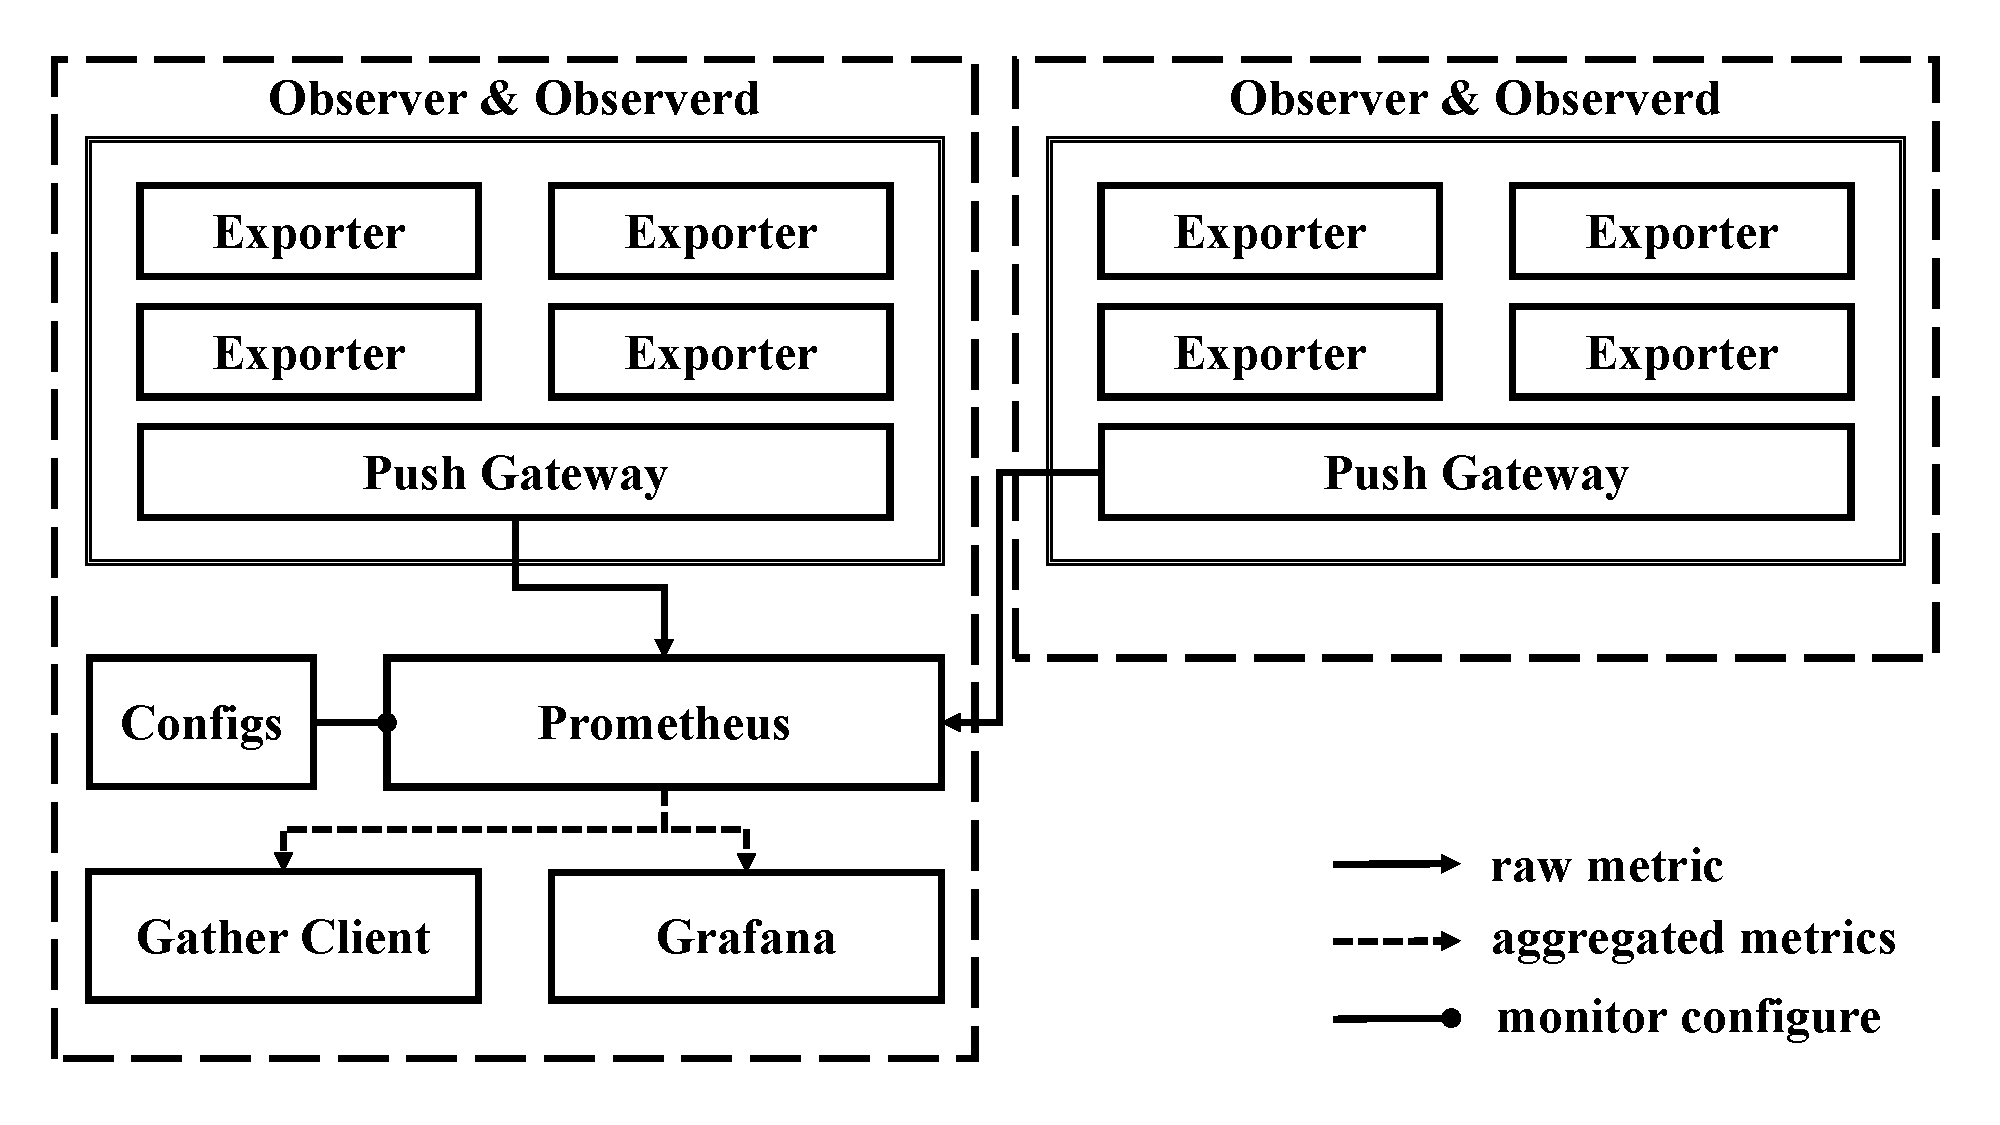
\includegraphics[width=0.8\textwidth]{monitor_arch}
    \bicaption{\quad 采集系统架构}{\quad Metric Collection System Architecture}
    \label{fig:monitor_arch}
\end{figure}

本研究结合云原生的实践经验,选择基于Prometheus来实现可观测性系统。Prometheus\citep{prometheus}是云厂商中广泛使用的一种指标监测系统,具有可扩展性强、灵活性好、生态丰富、部署便捷等特点,Prometheus的核心贡献在于提供了一种扩展性强的时序数据结构Metric以及围绕Metric的PromQL向量查询语言、向量数据存储方式以及编解码机制,在此基础上,Prometheus还实现了一套采集系统,提供了Promethues Server、Grafana及Node Exporter等核心组件,由于Promethues完全开源并提供了各种语言的Metric采集基础库,因此吸引了大量开发者及云厂商的参与,催生出丰富的组件生态。当前Prometheus已经成为指标采集的主要标准,并随DevOps的发展被越来越广泛地使用。

基于Prometheus生态的实时可观测性系统架构如图~\ref{fig:monitor_arch}所示,其中Observer的基于Prometheus Server与Grafana标准组件实现,在向量数据存储上,将原生的TiDB替换位InfluxDB,InfluDB使用以Rust语言编写,性能更强、扩展性更好。在采集上,Observer中虚拟机各维度数据的采集组织为一个服务发现配置文件,基于Prometheus的服务发现规则编写。而在数据聚合上,各维度原始数据首先需要进行初步处理以生成有效数据,Observer提供了PromQL编写了基本的聚合规则,实现对于标量数据的变化速率、99分位数据等的统计,同时这些规则会转化为Grafana中的Dashboard以进行实时监测。

可观测性系统中Observed的实现则包含了各个维度的Exporter的开发与配置。如图~\ref{fig:exporters}所示,Observed中包含了6种Exporter,能够在Host、Hypervisor、App三个维度围绕虚拟机提供丰富的数据采集,原始指标如表~\ref{tab:metric_list}所示,包含CPU、Cache、Memroy、IO、Network等各个子系统,总数量达到344个。

\begin{figure}[!htbp]
    \centering
    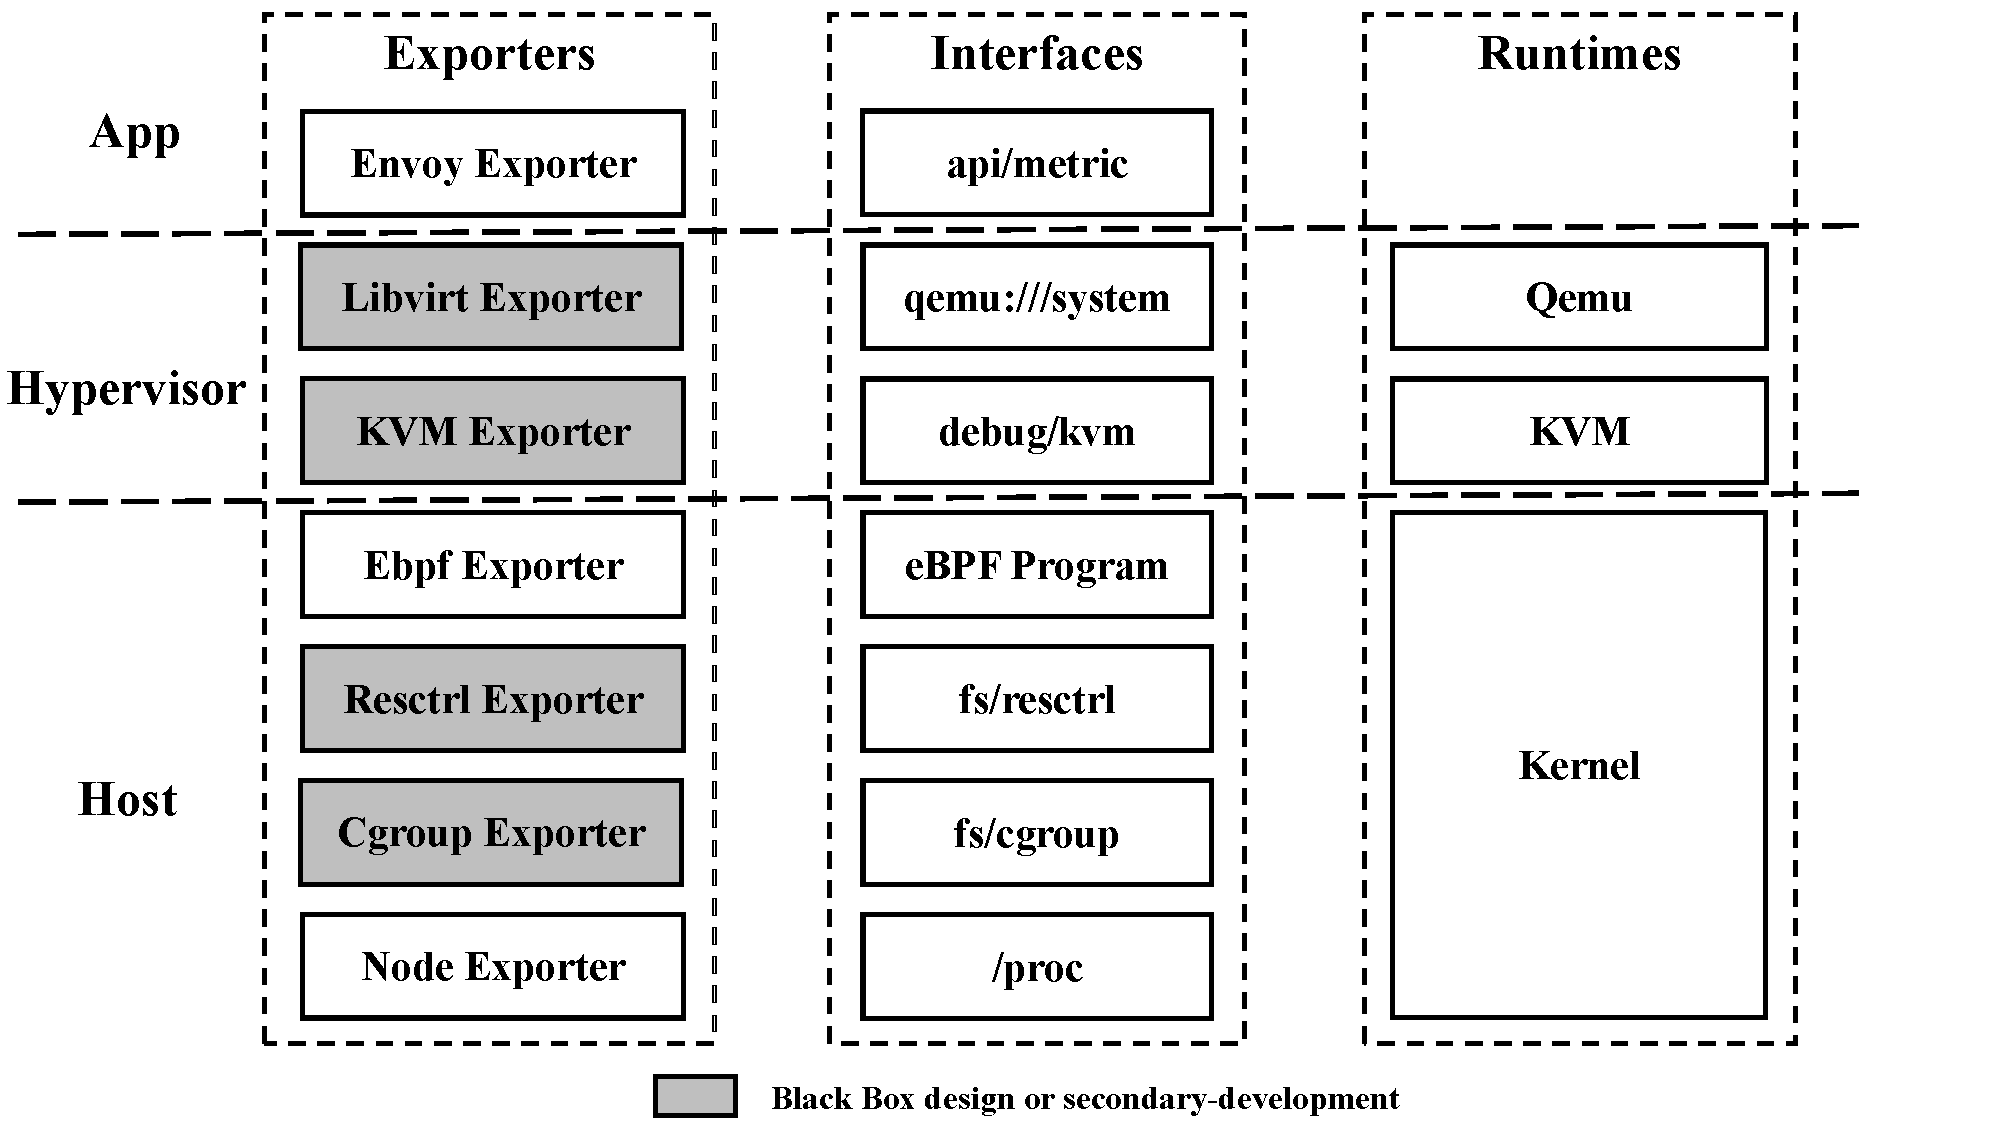
\includegraphics[width=0.9\textwidth]{exporters}
    \bicaption{\quad Exporters设计}{\quad Exporters Design}
    \label{fig:exporters} 
\end{figure}

1)Node Exporter是Prometheus提供的基础监控组件,提供Host维度的基础指标采集。其实现中主要利用了Linux Kernel提供的交互结果,来获取Host各个子系统中的运行状态信息,如通过/proc内核文件系统,获取运行时间、内存信息等。Observed实现中使能了NodeExporter的Perf Event监测模块,模块支持采集Host上的性能事件,包括cycles、instruction及cache miss等。

2)Resctrl Exporter实现了Resctrl子系统的指标采集。Intel RDT等硬件技术提供了进程粒度的CPU末级缓存与内存带宽的监测能力,Linux Resctrl作为这类技术的软件接口,提供了一个内核文件系统,用户可以通过在此文件系统中创建文件夹的形式来创建Monitor Group,而将进程加入到其中之后,Resctrl子系统就会开始为进程记录LLC与内存带宽信息。Resctrl Exporter基于Resctrl子系统实现, 通过扫描子系统中的Monitor Group来生成相关的指标信息,并将Monitor Group作为标签以便于后续聚合。

3)KVM Exporter实现了Hypervisor维度的指标采集。KVM内核模块提供了一个Debug文件系统,在最顶层的目录中,记录了内核模块的运行信息,如虚拟机陷出的总计数等,同时,对于每个虚拟机进程,还会创建对应的子目录,并以单个虚拟机为粒度记录内核模块的运行数据,最后,在每个虚拟机目录中,还会为每个vCPU创建一个目录,记录vCPU的时钟源相关信息。KVM Exporter基于上述机制实现,通过扫描Debug系统中的目录,并为遍历每个虚拟机条目来生成相关的指标信息,默认情况下使用虚拟机进程号作为标签,也允许传入一个配置文件,来实现虚拟机进程号与虚拟机名称之间的转化。

4)Libvirt Exporter是社区开发的一个监控组件,提供了Hypervisor维度的指标采集。Libvirt是一个统一的虚拟化接口层,提供了丰富的虚拟机管理选项,Libvirt Exporter基于Libvirt Monitor接口实现,能够采集虚拟机的各个设备的性能指标,如vCPU时间片、内存使用量、网络设备的吞吐量及IO设备的吞吐量等。Observed实现中为Libvirt Exporter增加的Perf Event监测功能,从而能够提供虚拟机粒度的性能事件指标信息,如cycles、instruction及cache miss等。

\begin{figure}[!htbp]
    \centering
    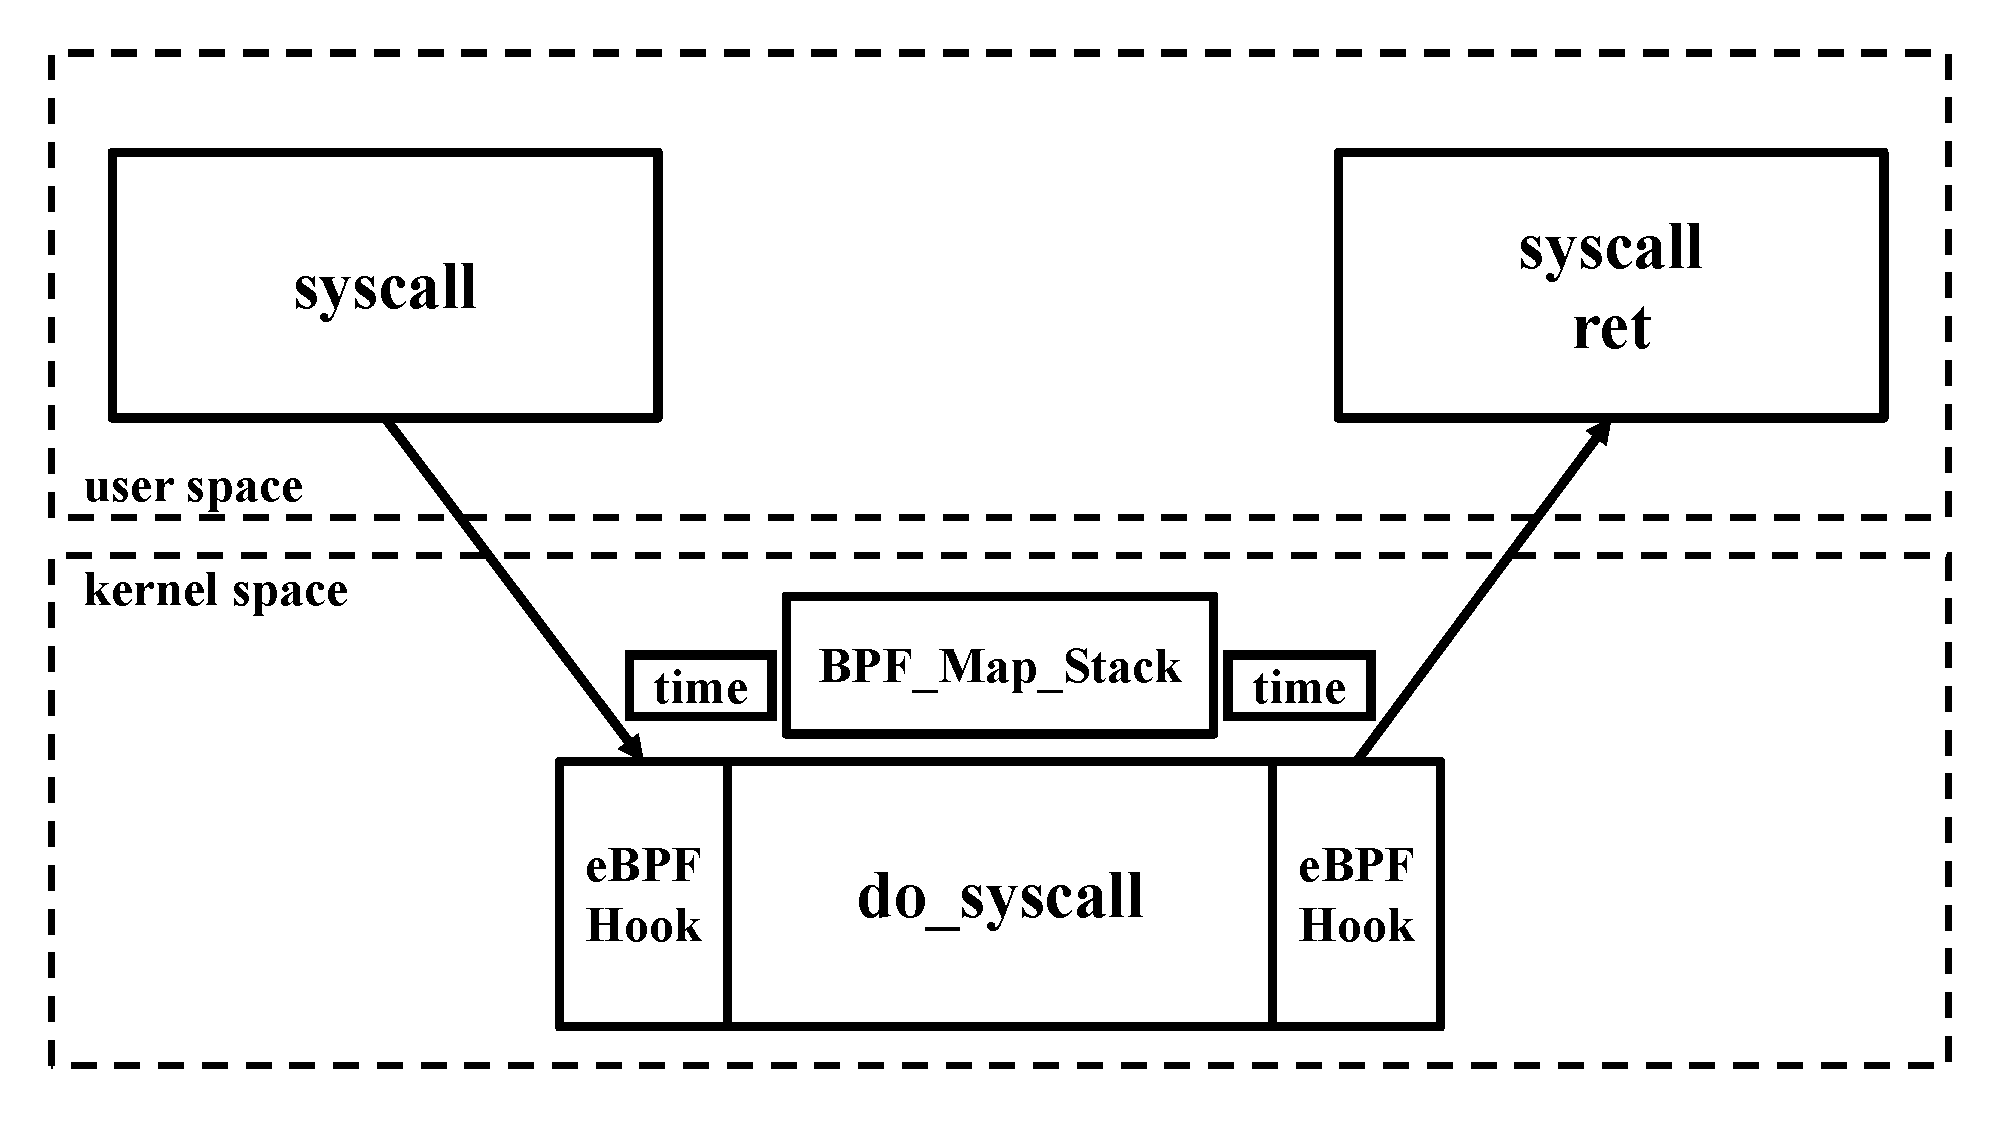
\includegraphics[width=0.7\textwidth]{syscall_hook}
    \bicaption{\quad eBPF Syscall插桩}{\quad eBPF Syscall Hooking}
    \label{fig:syscall_hook}
\end{figure}

5)eBPF Exporter是社区开发的一个监控组件, 提供了内核侧的自定义指标采集。eBPF Exporter能够加载用户编译为字节码的eBPF程序,并通过RingBuffer收集内核侧eBPF程序采集的数据转化为指标。Observed中实现了系统调用及vHost Net内核模块两个eBPF采集程序。内核中系统调用分布在各个子模块中,并通过注册系统调用的方式加入到系统调用表中,用户态应用发起的系统调用会触发一次中断,并最终进入系统调用分发函数,因此可以利用raw tracepoint机制在系统调用分发函数的开始与结束处进行eBPF插桩,如图~\ref{fig:syscall_hook}所示,每当进程进入系统调用中时,首先可以通过BPF Helper函数获取当前task结构体指针,并读取进程号等标识信息,其次通过读取系统调用上下文中的ax寄存器,来获取当前的系统调用号,这两个信息提供了基本的指标标签,基同时,利用BPF Stack来记录时间戳信息,就能够在系统调用返回时计算整个系统调用的执行时间,从而实现对于而对进程每个系统调用吞吐、延迟的监测。vHost Net内核模块的监测则围绕worker内核线程展开,如图~\ref{fig:vhost_net}所示,worker线程中可能执行4种不同的回调函数,分别用于虚拟机的网络发送与接受,通fentry机制过在这些函数的入口与出口出进行插桩,就能够统计出各个函数执行频率以及延时等信息。

\begin{table}[H]
    \bicaption{\quad 指标列表}{\quad Metric list}% caption
    \label{tab:metric_list}
    \footnotesize% fontsize
    \setlength{\tabcolsep}{4pt}% column separation
    \renewcommand{\arraystretch}{1.5}% ro w space 
    \centering
    \begin{tabular}{lcc}
        \hline
        %\multicolumn{num_of_cols_to_merge}{alignment}{contents} \\
        %\cline{i-j}% partial hline from column i to column j
        层级 & 来源 & 指标\\
        \hline
        Host & Kernel(271) & [cpu] sys\_time、user\_time、freq ... \\
        & & [mem] usage、avail、swapfree、bounce、hugepage ...\\
        & & [network] transmit、netstat、sockstat、ip、speed ...\\
        & & [disk]flush requests、flush request time、read、write ...\\
        & & ...\\
        & eBPF(2) & [syscall] count、duration\\
        & Resctrl(3) & llc cap、mem b/w local、mem b/w total\\
        Hypervisor & Libvirt(68) & [vcpu] sys\_time、user\_time、wait、delay...\\
        & & [mem] usable、avail、dick cache、rss ...\\
        & & [perf] cycle、instruction、cache miss ...\\
        & & [block] flush request、flush time、read、write ...\\
        & & [interface] receive、transmit ...\\
        & & ...\\
        & KVM(59) & vm\_exit、io\_exit、irq\_exit、irq\_inject、halt\_poll ...\\
        App & Log/Envoy & qos, latency, rate, score ...\\
        \hline
    \end{tabular}
\end{table}

\section{实验设计}

\subsection{基准性能实验}

实验中使用两台C6服务器作为Client和Server,服务器具体配置如表~\ref{tab:c6_info}所示,其中Client服务器额外承担实验管理的功能,同时作为Observer角色部署Prometheus Server等组件,而Server主要承载具体的应用,同时作为Observed角色部署上述设计实现的6种Exporter,并为Exporter设置Numa亲和性以避免对应用产生干扰。基准性能实验测试无干扰情况下各个应用的基础性能,对于每个典型应用,使用华为云提供的竖亥Benchmark中的模拟负载多样的负载来监测不同场景下的基准性能。

\begin{table}[H]
    \bicaption{\quad C6服务器信息}{\quad C6 Information}% caption
    \label{tab:c6_info}
    \footnotesize% fontsize
    \setlength{\tabcolsep}{4pt}% column separation
    \renewcommand{\arraystretch}{1.5}% row space 
    \centering
    \begin{tabular}{lc}
        \hline
        类型 & 信息 \\
        \hline
        OS & Ubuntu 22.04 ( Kernel 5.15.0) \\
        CPU & Intel Xeon Gold 6151 (18 cores) * 2 \\
        Processor Core Frequency & 3GHz,Turbo 3.4GHz \\
        L1 Caches & 32KB *,  8-way set associative, split D/I \\
        L2 Caches & 1024KB, 16-way set associative \\
        L3 Caches & 25344KB, 11-way set associative \\
        Main Memory & 32GB * 12, 2666MHz DDR4 \\
        Storage & Avago MegaRAID, 2.18T SAS RAID0, 87.322T SATA RAID0 \\
        NIC & Intel Corporation Ethernet Connection X722 for 10GbE SFP+(10Gbit) \\
        \hline
    \end{tabular}
\end{table}

% 1)Redis、Memcached。使用memtier_benchmark来产生负载,负载的模型由华为云提供,包括Normal、Random两类模拟负载

% 2)Mysql。使用TPCC作为基准实验负载

% 3)Elasticsearch。使用YCSB作为基准负载

% 4)Kafka。

% 5)Nginx。

% 6)Render。使用华为内部的模拟负载。

\subsection{性能劣化实验}

% 干扰应用
% - 干扰有效性
% - 噪声控制

性能劣化实验通过增加目标应用与干扰应用的混部场景,分析应用对于不同干扰类型的敏感程度。在干扰应用的选择上,使用stress-ng来产生不同类型的干扰。stress-ng是Linux系统中常用的压力测试工具,能够模拟各种资源的压力场景,而实验中则利用其模拟各种压力场景的特性来制造干扰,并观测目标应用的性能劣化情况。stress-ng提供了丰富的配置参数,本课题选用如表~\ref{tab:arg_list}所示的参数配置,来制造CPU、Cache、内存、IO、Network上的干扰。

\begin{table}[H]
    \bicaption{\quad stress\_ng 实验参数列表}{\quad stress\_ng args list}% caption
    \label{tab:arg_list}
    \footnotesize% fontsize
    \setlength{\tabcolsep}{4pt}% column separation
    \renewcommand{\arraystretch}{1.5}% row space 
    \centering
    \begin{tabular}{lcc}
        \hline
        %\multicolumn{num_of_cols_to_merge}{alignment}{contents} \\
        %\cline{i-j}% partial hline from column i to column j
        子系统 & 参数 & 说明\\
        \hline
        CPU	    & --cpu & 循环执行sqrt(rand())的线程数量\\
	            & --cpu-load & 线程负载的比率\\
        Cache	& --cache & cache抖动线程数量\\
	            & --cache-level	&测试指定等级的Cache\\
	            & --icache	&指令cache抖动的线程数量\\
        IO	    & --io	&循环执行sync()的线程数量\\
	            & --iomix	&执行混合I/O操作的线程数量\\
	            & --hdd	&循环执行write()/unlink()的线程数量\\
	            & --seek	&执行随机seek I/O的线程数量\\
        Memory	& --vm	&循环执行匿名mmap的线程数量\\
	            & --vm-bytes	&执行vm操作的buffer大小\\
	            & --memrate	&执行read/writes的线程数量\\
	            & --memrate-bytes	&执行内存操作的buffer大小\\
	            & --malloc	&执行malloc/realloc/free的线程数量\\
	            & --memcpy	&执行memory copy的线程数量\\
        Network	& --sock	&执行Socket I/O的线程数量\\
	            & --epoll	&执行epoll处理的线程数量\\
        \hline
    \end{tabular}
\end{table}

正式干扰实验之前,首先需要验证干扰的效果。测试实验使用一个4 CPU 8G Memory虚拟机,并在其中按照上述配置运行stress-ng干扰应用。干扰强度的定义与配置的stress-ng线程相关,对于CPU干扰,采用线性的干扰强度,即干扰强度正比于CPU负载,而对于其他干扰则使用指数映射,即干扰强度与线程数量呈指数关系,以便于快速探测干扰峰值。具体实验的结果从可观测性系统中获取,每种干扰选择一个表征指标用以说明,具体结果如图~\ref{fig:interference}所示。

1)CPU干扰选择CPU Usage作为表征指标,干扰效果如~\ref{fig:cpu_interference}所示,可见随干扰强度的不断提升,干扰应用逐渐能够占用所有的核心资源。

2)Cache干扰选择Cache Usage作为表征指标,干扰效果如图~\ref{fig:cache_interference}所示,可见随干扰强度的不断上升,干扰应用逐渐能够占用全部的LLC。同时,当干扰强度上升至5之后,Cache Usage就几乎稳定在峰值。

3)IO干扰选择IO Input Bytes作为表征指标,干扰效果如图~\ref{fig:io_interference}所示,在前段,随干扰强度的上升,干扰应用占用越来越多的IO带宽,但当干扰强度超过5之后,干扰应用占用的IO带宽反而开始减少。由于IO干扰强度与干扰线程数量指数相关,高干扰强度下会产生大量的IO线程,这些线程彼此之间会相互竞争,因此导致整体的IO带宽下降。

\begin{figure}[H]
  \centering
  \begin{subfigure}[b]{0.45\textwidth}
    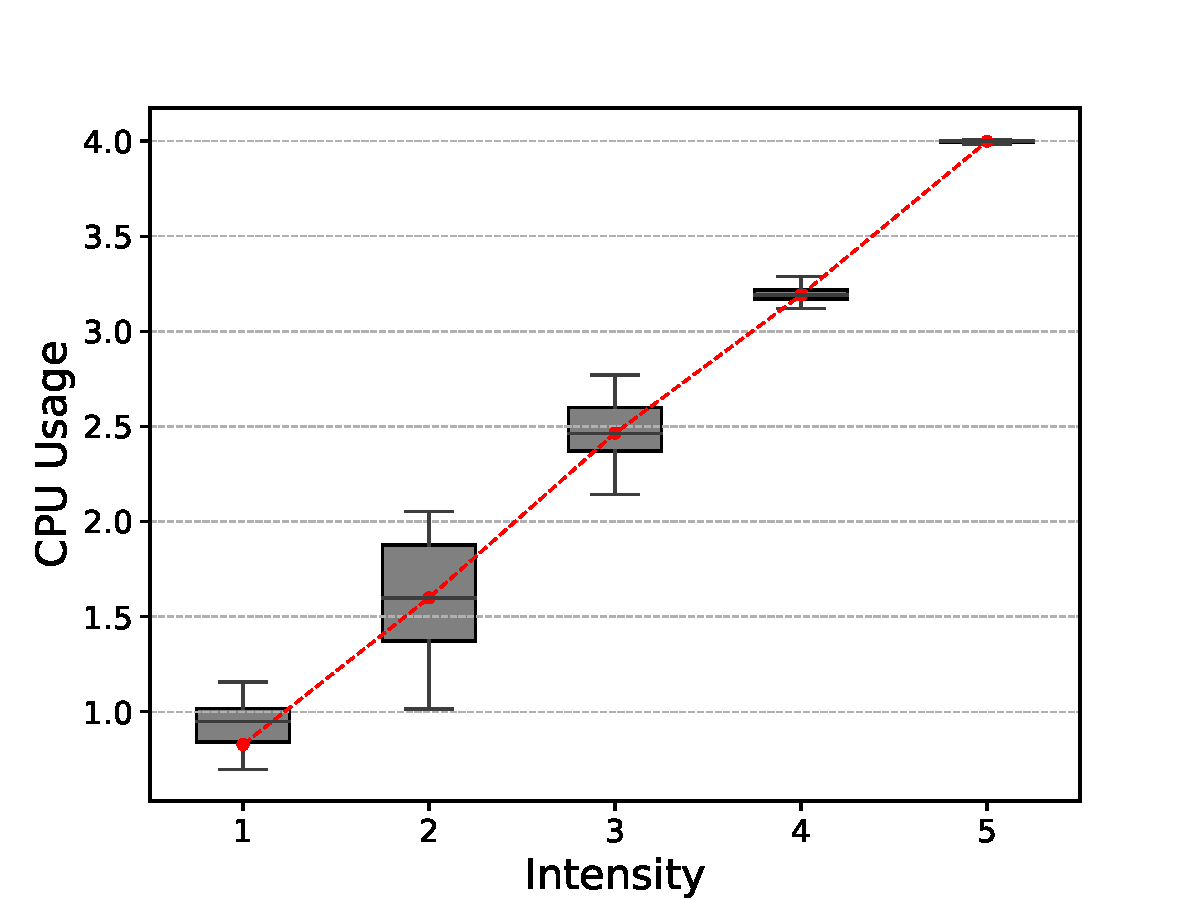
\includegraphics[width=\textwidth]{cpu_interference}
    \caption{cpu干扰效果}
    \label{fig:cpu_interference}
  \end{subfigure}
  \begin{subfigure}[b]{0.45\textwidth}
    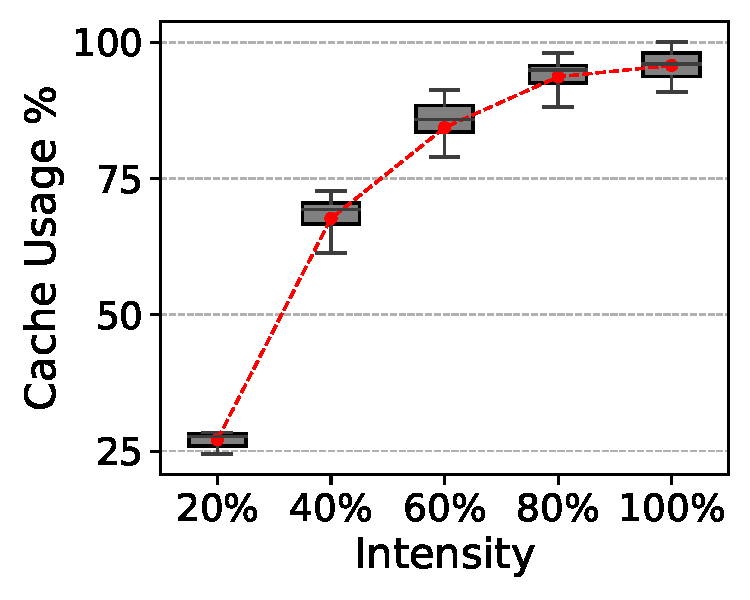
\includegraphics[width=\textwidth]{cache_interference}
    \caption{cache干扰效果}
    \label{fig:cache_interference}
  \end{subfigure}
  \begin{subfigure}[b]{0.45\textwidth}
    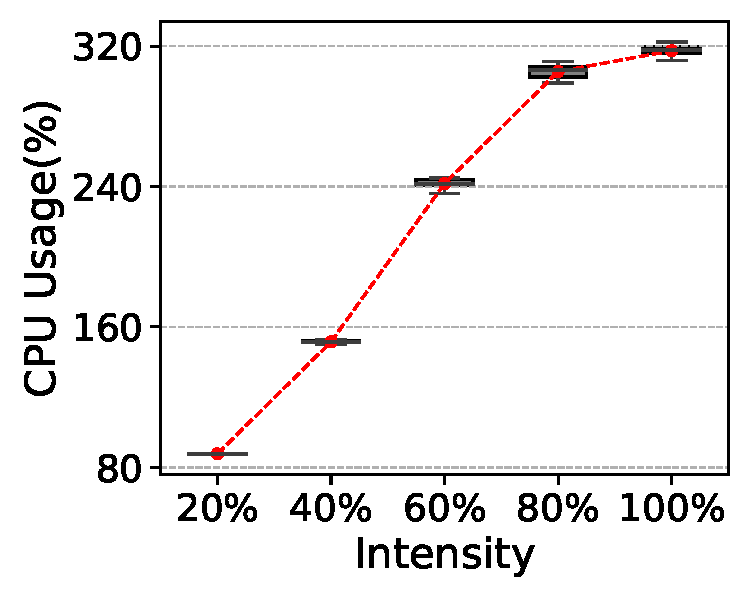
\includegraphics[width=\textwidth]{io_interference}
    \caption{io干扰效果}
    \label{fig:io_interference}
  \end{subfigure}
  \begin{subfigure}[b]{0.45\textwidth}
    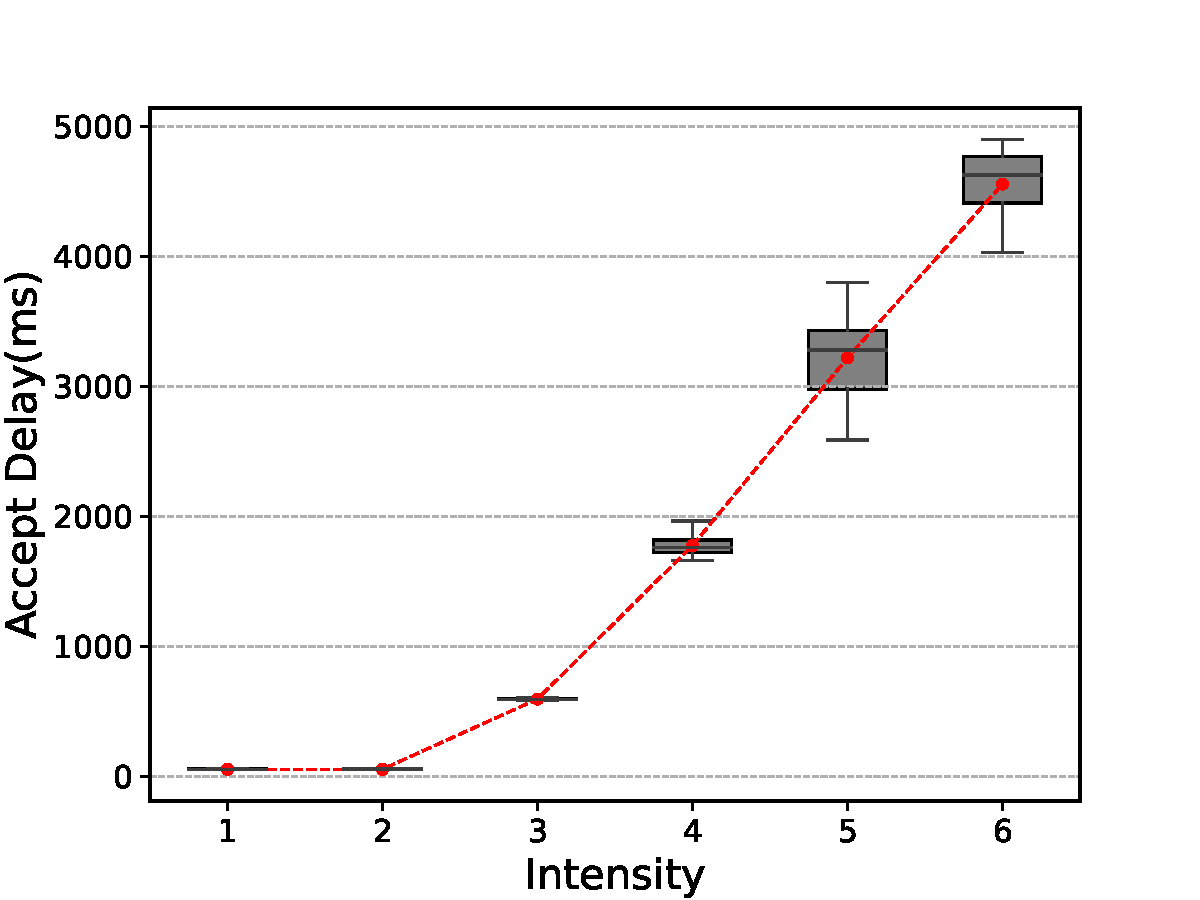
\includegraphics[width=\textwidth]{net_interference}
    \caption{net干扰效果}
    \label{fig:net_interference}
  \end{subfigure}
  \caption{干扰效果}
  \begin{subfigure}[b]{0.45\textwidth}
    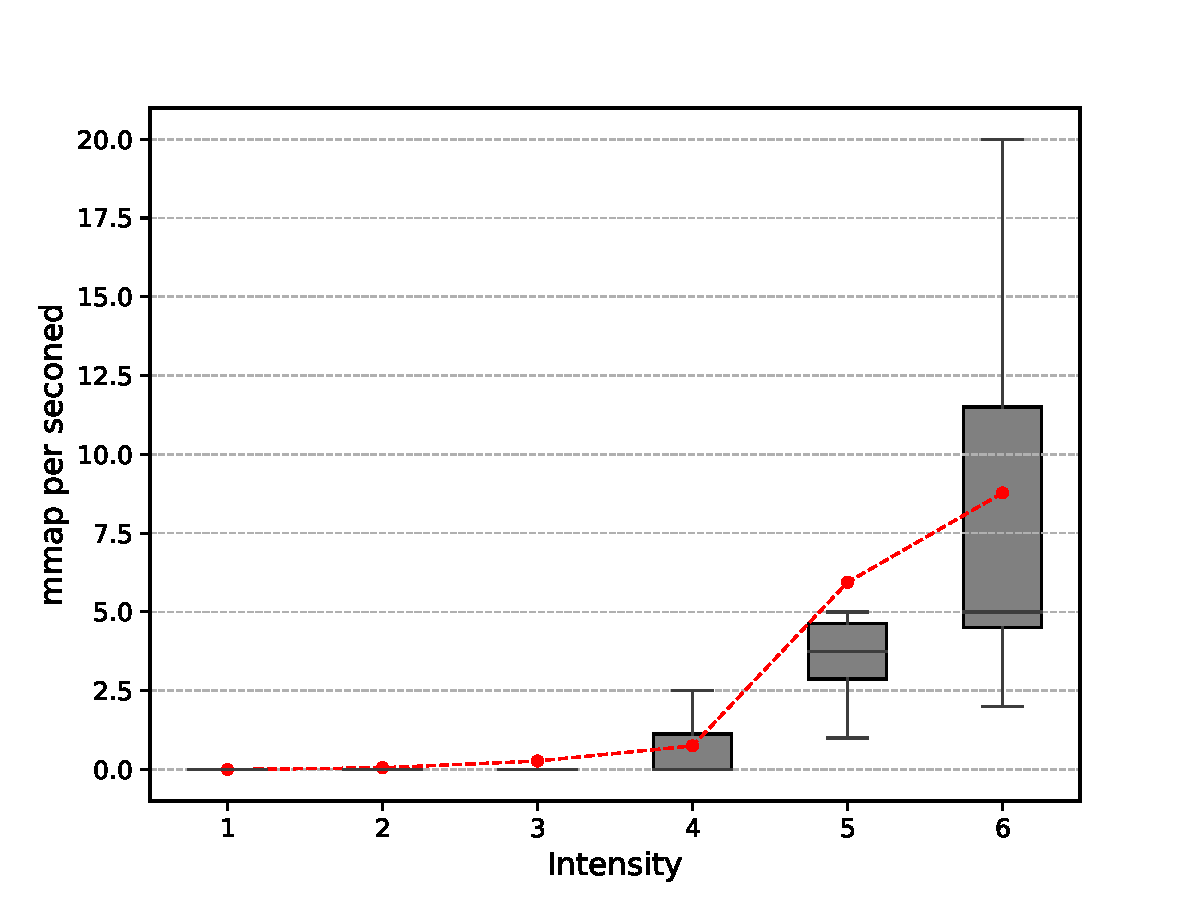
\includegraphics[width=\textwidth]{vm_interference}
    \caption{内存干扰效果}
    \label{fig:vm_interference}
  \end{subfigure}
  \label{fig:interference}
\end{figure}

4)Net干扰选择Accept系统调用延迟作为表征指标。Accept系统调用通常发生在Server类应用中,用于与Client建立连接,Accept系统调用变慢通常意味着连接排队延迟与客户端超时,而具体的干扰效果如图~\ref{fig:net_interference}所示,可见随干扰强度的不断上升,Accept系统调用的延迟逐渐变大,由于延迟指标可以无限增加,实验中根据应用延迟范围来确定干扰强度。

5)Memory干扰使用每秒的mmap系统调用次数作为表征指标。stress-ng通过频繁地调用mmap来产生内存干扰,如图~\ref{fig:vm_interference}所示,随干扰强度的上升,每秒的mmap系统调用数量也在不断上升,并在干扰强度为6时出现较大的波动。

\section{画像分析与结论}

\subsection{典型应用资源使用倾向分析}

无干扰实验中,不同应用对应的资源指标如图~\ref{}所示。从整体上看,Block I/O与Network I/O两类指标在不同应用之间呈现出较大的差异,相同指标在不同应用中的极大值与极小值差异可达104~105倍,而其余指标的差异通常不会超过20倍,这就导致图中一部分应用I/O相关指标非常高,而另一部分应用的相同指标则始终为一个较低的值。而在其他指标上则没有体现明显的差异度,这有如下两方面原因,首先,对于"利用率"类型的指标,这些指标存在明确的上下界,同时数值上的差异度难以直接体现,如对于CPU利用率,80\%与90\%利用率仅有约12\%的数值差异,但计算空闲CPU占比,则前者是后者的200\%,对于这些指标不能简单地使用差异度度量。其次,一些与硬件相关的指标波动不明显,如CPI,其波动通常受到流水线周期、指令阻塞和回退的数量等因素影响,在优化较好的现代处理器平台上,通常只会在一个较小的范围内波动。

具体到应用的差异性如图~\ref{}所示,不同应用对于主要的5种系统资源的需求呈现处较大的差异:

1)CPU资源:应用的运行都需要CPU资源, 而不同应用对于CPU资源的使用上存在差异。Kafka运行时需要较多的CPU资源,体现在较高的IPS指标上。Redis、Memcached同样对于CPU资源有较高需求,从较多的平均CPU时间片占用能够看出,但不同之处在于,Redis、Memcached对于CPU资源的使用与请求强相关,在请求量较低时,由于频繁的睡眠与唤醒,此时不仅CPU资源需求少,同时CPI也较高,而当请求量足够多时,由于都基于epoll实现,因此密集的请求使得两者总是能够保持CPU的占用,而相较于Redis,Memcached在默认配置下更能够利用多核优势。Render应用同样需要较多的CPU资源,但与上述应用不同的是,Render在CPU资源使用上相当稳定,这一特点反映在较低的Branch IPS及Context Switch指标上。

2)Cache资源:末级缓存资源与内存访问强相关,分析不同应用的LLC相关指标,可以将应用按访存局部性进行划分,其中Niginx属于局部性较好的应用,其在运行过程中LLC使用率波动不明显,并且LLC Miss数量较少。而对于Redis、Memcached这类键值存储型应用,局部性则与工作负载相关,在随机负载下局部性表现较差,而在模拟负载下局部性则相对较好。

3)Memory资源:内存资源区分带宽与使用量。典型应用中,Nginx在模拟负载下对内存带宽的需求较高,这点与其在Cache资源需求上的表现一致,而其余应用则采用间歇与分批的内存读取,因此不会占用过多的内存带宽。而在内存使用量上,典型应用的内存占用除自身所需外,都与工作负载相关,而在华为云的默认负载下,各个应用都会占用一定量的内存而并没有特别的规律性。

4)Network资源:在网络资源上,不同的应用使用需求差异很大,其中Redis、Memcached、Kafka表现出极高的网络需求,事实上这些应用都是服务型应用或自身就是网络消息中间件。而Elasticsearch、Render等在网络资源的需求上则相对较少,其中Elasticsearch并非不使用网络,而因为工作负载中并没有长时间且持续性的请求,Render则因为是离线应用,因此几乎不会使用到网络资源。

5)I/O资源:在I/O资源上,不同应用的使用需求差异同样十分大。其中Elasticsearch、Kafka和Mysql由于涉及到存储内容的持久化,因此会大量地使用I/O资源。而类似Redis等应用,虽然存在数据持久化的配置,但实际运行中持久化频率较低,因此通常只会有周期性的少量I/O资源占用。

\subsection{典型应用资源敏感度分析}

资源敏感度主要分析典型应用与不同配置下的干扰进行混部后的性能劣化情况,其中应用性能使用竖亥Benchmark提供的白盒指标进行评价。白盒指标中既有经过加权计算后的统一评分,也有对于每个应用单独的评价指标,在性能劣化中,主要选择劣化程度与干扰程度较为相关的指标进行分析。不同应用核心性能指标与干扰强度的关系如图~\ref{}所示,而综合图例结果分析能够将应用分为以下4类:

1)单纯CPU敏感型:此类应用对于CPU干扰最为敏感,而受其他干扰影响的程度则明显更低。如Memcached,其在受到CPU资源干扰后产生了近50\%的性能劣化,而对于在其他干扰下的劣化程度则在10\%内,同样的情况也在Kafka的实验数据中出现。

2)CPU与Cache敏感型:此类应用同时受CPU与Cache干扰明显,且通常对CPU干扰更加敏感。如Redis,与Memcached类似,对CPU干扰十分敏感,而同时由于Redis没有开启多线程支持,因此在Cache资源上的竞争能力弱于Memcached,从而更容易受到Cache干扰的影响。Elasticsearch情况则更为复杂,竖亥Benchmark中提供了不同的白盒指标来表征Elasticsearch的性能,主要分为吞吐量与延迟,以吞吐量作为标准,则Elasticsearch符合CPU敏感型,而以延迟作为标准,则Elasticsearch则更倾向于CPU和Cache敏感型,这种现象在其他典型应用中也有出现,而对于Elasticsearch,其使用场景中更注重吞吐量,因此在本研究中将其归类为CPU与Cache敏感型。

3)资源不敏感型:此类应用对于所有干扰的敏感度都偏低。实验中Render在各个干扰下都没有出现较为明显的劣化,这主要有两个原因。一方面,在性能指标上,Render应用使用了完成时间作为性能评价指标,而与其他应用的性能指标不同,完成时间这一指标更偏向于整个运行过程的总体性能述而不是单一处理过程的性能,一些突发的性能劣化不会体现在这一指标上,另一方面,内核调度机制上在未作限制时倾向于公平地分配时间,因此干扰程序会因调度的影响向Render出让CPU时间,而当CPU资源总和足够满足Render使用时,性能指标就不会出现较大变化。

\section{本章小结}

本章主要论述了对应用进行画像分析的过程,首先结合与云厂商的合作经验,确定了在以虚拟机为沙箱环境运行有限个应用的场景,并选取了云场景中常见的7种应用作为画像分析的对象。

然后对场景进行拆解分析,并提出了一种从Host、Hypervisor到App三个层次的协同监控机制设计,利用虚拟机本身作为进程的特殊性,串联三个维度的指标,并创新性地提出了一种基于eBPF对虚拟机监测的方式,对于本身为进程的虚拟机,监测其在系统调用上的吞吐与延时,而针对虚拟机的特殊性,则通过在虚拟化设备后端的关键路径上进行监测,实现更丰富的指标采集。

随后根据上述设计,设计实现了一套可观测性系统,除利用到开源的Promethues、Node Exporter外,还根据监控需要,实现了Libvirt Exporter、KVM Exporetr、Resctrl Exporter以及Kernel Exporter,完成所有的设计需求。

在可观测性基础设施实现完毕后,本章继续讨论实验的设计,实验围绕8种常见应用展开,并设计了有干扰实验与无干扰实验,在有干扰实验中,利用资源限制手段来减少干扰中的噪声,通过制造CPU、Cache、Memory及IO四种干扰,来分析应用对于干扰的敏感程度,而通过无干扰实验,来分析应用的资源使用倾向

最后在所有实验完成之后,分析从Prometheus中采集得到数据,来为应用进行画像分析,提供了应用的资源使用倾向及干扰敏感度评级,并探讨了除LC与BE外更多的混部机会。